\section{Image Reconstruction for MeerKAT} \label{intro}
%Ill-posed Inverse Problems

In Signal Processing, we have the problem of reconstructing the measured signal from noisy measurements. on topics like image reconstruction, we want to remove the instrumental effects of measurements and retrieve the truly observed image. 

Image reconstruction problem appear in astronomy, where we want to account for effects like atmosphere, or gravitational lensing. In Radio Interferometry, Image reconstruction is an active field of research. The new MeerKAT Interferometer poses new challenges for image reconstruction. 

This project focuses on image reconstruction for radio interferometers by using compressed sensing. But the basic principles would also apply for different setups, like MRI scans.

The basic measurement equation does not look threatening \eqref{intro:measurement}. 

\begin{equation}\label{intro:measurement}
V(u, v) = \int\int I(x, y) e^{2 \pi i (ux+vy)} \: dx \: dy
\end{equation}

The Interferometer measures Fourier Components $V$ of the sky image $I$ (called Visibilities in Radio Astronomy). The task is to reconstruct the actual image of the sky $I$. On first glance, this problem can be solved by using the two dimensional Fourier Transform. But two properties of the measurements make this harder:
\begin{enumerate}
	\item Non-uniform sampling pattern in Visibility space
	\item Incomplete Measurements. 
\end{enumerate}


Problems of non uniform samples is that we cannot use the Fast Fourier Transform. We can still use the naiive fourier transform, but the data We are interested in an image $X$ with uniformly sized pixels. The instrument measures areas in Visibility space more densely than others. This property keeps us away from the Fast Fourier Transform. The inverse Fourier Transform can still be calculated, but it results in an algorithm with quadratic runtime. It is not practical

Incomplete measurements create wrong artefacts in the image. Reconstructing the image is finding out which structures are plausible and which are not. Generally an ill-posed inverse problem, meaning: It may not have a unique solution, small changes in measurements lead to large changes in the image.  CLEAN class of Algorithms that approximate a solution. The standard implementation.

Applying the theory of compressed sensing to certain reconstruction problems, because they are we have theoretical guarantees with them. 
Compressed Sensing\cite{candes2006robust}\cite{donoho2006compressed} reconstructions useful for incomplete measurements. It has been successfully applied to image reconstruction for radio interferometers with algorithms like SASIR \cite{starck2015starlet} or more recently reconstructions using SARA \cite{dabbech2018cygnus} \cite{birdi2018sparse}


Current algorithms solve these two problems all the same way. They use the major cycle architecture.


\subsection{The Major Cycle Architecture}
The major cycle architecture was conceived for the CLEAN class of algorithm. Compressed sensing approaches use essentially the same architecture. The figure \ref{intro:major} shows the major cycle framework. In a major cycle consists of two parts: The non-uniform FFT and an optimization algorithm.

Together, they form the major cycle which solves the two problems over several iterations. In the end, we have an estimate over which part of the visibilities is noise.

\begin{wrapfigure}{r}{0.6\textwidth}
	\centering
	\vspace{-10pt}
	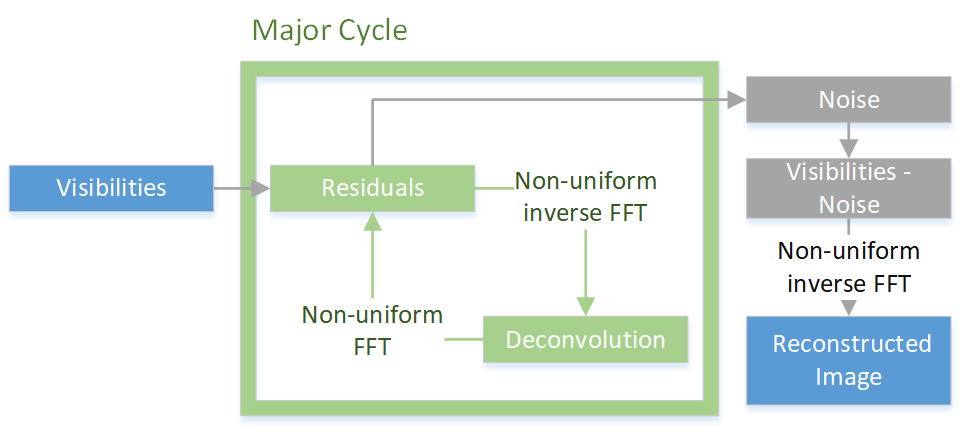
\includegraphics[width=1.0\linewidth]{./chapters/01.intro/Major-Minor.png}
	\caption{The Major Cycle Framework}
	\label{intro:major}
	\vspace{-10pt}
\end{wrapfigure}

The non-uniform FFT is responsible for approximating a regularly spaced image from the measurements, and for approximating the measurements corresponding to an image. Non-uniform FFT's are fast approximation algorithms, but by being approximation algorithms, they introduce errors. 

A optimization algorithm uses the image and removes the effect of incomplete samples. In the past, CLEAN algorithms were used to remove the effects. For the future, algorithms based on the theory of compressed sensing show promises in image quality.

A full major cycle consists of the following operations: First, it approximates the regularly spaced the regularly spaced image from the measurements. Then the optimization algorithm removes the effects of Incomplete measurements and returns the corresponding image. The major cycle then approximates the measurements corresponding to the image with the non-uniform FFT. The residual measurements are used in the next Major Cycle. In each cycle, two errors get simultaneously reduced:

\begin{enumerate}
	\item The Error introduced by the non-uniform FFT.
	\item The Error introduced by the incomplete measurements.
\end{enumerate}

After several major cycles the algorithm converges on a regularly spaced image which has a small error from non-uniform samples, and a small error from incomplete measurements.

For the optimization algorithm, the CLEAN class of algorithms get used. But algorithms based on the theory of compressed sensing have been shown to produce superior images.


\subsection{Compressed Sensing Reconstructions}
 However, compressed Sensing algorithms come with the drawback of requiring more major cycles.

MeerKAT due to wide field of view introduces even more troubles

Current Compressed Sensing reconstructions reduce the number of major cycles. However, the question is if Compressed Sensing can use a different architecture, and scale better to problems of the size of MeerKAT.

Furthermore on the new MeerKAT instruments, we have a big data problem. We want to create a large image from a large amount of Visibilities. 32k*32k pixels and terabytes of raw Visibility data. 

Scalability is a big problem.

There are ways to get rid of the major cycle, but overall the complexity could not be reduced.









